% Author: Izaak Neutelings (24/01/2023)
% PhD checklist: https://www.mnf.uzh.ch/en/studium/phd/checkliste-fuer-doktorierende.html
% UZH CMS wiki https://wiki.physik.uzh.ch/cms/newcomers:gettingstarted#phd_students
\RequirePackage{fix-cm} % against warnings for \fontsize
%\documentclass[a4paper,11pt]{book}
\documentclass[a4paper,11pt,usegeometry]{scrreprt} % scrreprt = KOMA script
\usepackage[T1]{fontenc} % load before inputenc
\usepackage[utf8]{inputenc}
%\usepackage{lmodern} % different font
\usepackage{tikz}
\usepackage{lipsum} % dummy text
\usepackage{setspace} % for \setstretch
\usepackage{geometry} % WARNING: add 'usegeometry' option for scrreprt class

% PAGE LAYOUT / MARGIN
\setlength{\topmargin}{-1.3cm}
\setlength{\oddsidemargin}{0.2cm}
\setlength{\evensidemargin}{0.2cm}
\setlength{\textheight}{25cm}
\setlength{\textwidth}{16cm}
\setlength{\footskip}{1.2cm} 
\setlength{\footnotesep}{0.4cm}

\begin{document}

% TITLE PAGE
% The layout of the title page for PhD dissertations at the MNF of UZH must be
% strictly adhered to. Do not change any of the spacing, line breaks, or font sizes!
% Keep the % characters at the end of text lines to avoid spurious spaces.
% For more information, please see
%   https://www.mnf.uzh.ch/en/studium/phd/checkliste-fuer-doktorierende.html
\newgeometry{margin=1cm}
\begin{titlepage}
\begin{center}
\setstretch{1} % unset (locally) any scaling of the linespacing

%% OVERLAY official title page from MS Word template of UZH MNF for fine-tuning the spacing
%\begin{tikzpicture}[remember picture,overlay] % use \usepackage{tikz} in the preamble
%  \node[draw=red,line width=10,fill opacity=0.2] at (current page.center){%
%    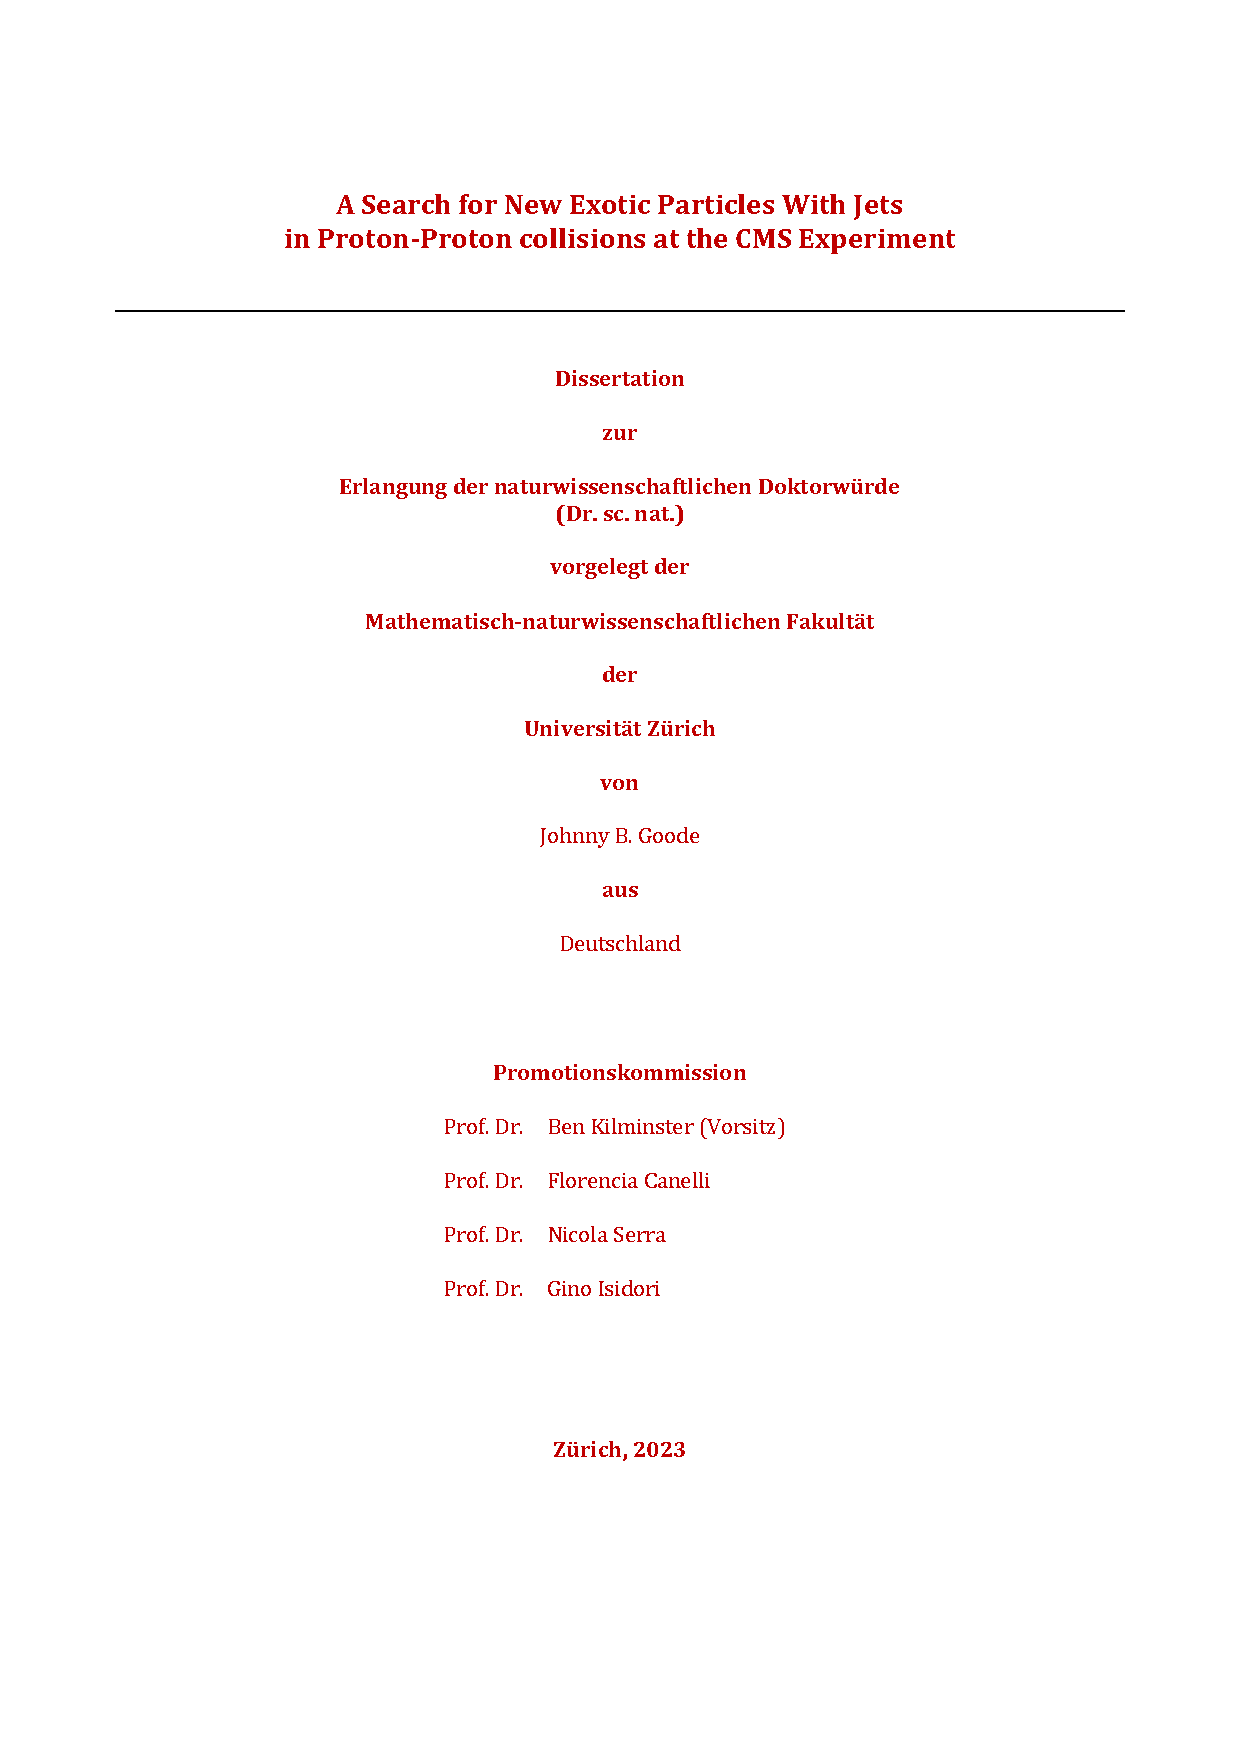
\includegraphics[scale=1]{titlepage_UZH_PhD_red.pdf}};
%\end{tikzpicture}

% TITLE
% Rules for capitalization in titles
% - Capitalize nouns, pronouns, verbs (including conjugated forms of to be), adjectives, and adverbs.
% - Lowercase definite and indefinite articles (a, an, the).
% - Lowercase all prepositions when used strictly as prepositions.
% - Capitalize prepositions when used as adverbs or adjectives: "Straighten Up and Fly Right".
% - Lowercase usage of “to” in all situations – whether as a preposition or as part of an infinitive.
% - Capitalize the second part of a hyphenated compound: "Research-Based Teaching and Learning".
\vspace*{\dimexpr-\topmargin-\headheight-6.4mm\relax}
\bfseries\fontsize{14pt}{17pt}\selectfont % bold font, 14pt
A Search for New Exotic Particles with Jets\\
in Proton-Proton Collisions at the CMS Experiment%

% HORIZONTAL LINE
\vspace{3pt}
\centerline{\rule{171mm}{0.3pt}} % horizontal line
\vspace{24pt}

% INSTITUTE
\bfseries\fontsize{11pt}{12.95pt}\selectfont % bold font, 11pt
Dissertation%
\break
\break
zur%
\break
\break
Erlangung der naturwissenschaftlichen Doktorw\"urde%
\break
(Dr. sc. nat.)%
\break
\break
vorgelegt der%
\break
\break
Mathematisch-naturwissenschaftlichen Fakult\"at%
\break
\break
der%
\break
\break
Universit\"at Z\"urich%
\break

% AUTHOR
% State your first name(s) in the form you prefer; at least one first name must be written out in full. 
% This information will be used for the doctorate diploma.
\bfseries % bold font
von%
\break
\break
\mdseries % medium font
Johnny B. Goode%
\break

% AUTHOR'S CITIZENSHIP
% If you have a Swiss citizenship use von and fill in your place of citizenship
% and your canton of citizenship, e.g., 'von Uster ZH'
% If you are not a Swiss citizen use aus and fill in the country you are from.
% e.g. 'aus Frankreich', 'aus der V.R. China'
\bfseries % bold font
%von% % for Swiss citizens
aus% % for non-Swiss citizens
\break
\break
\mdseries % medium font
%Genf GE%
%Uster ZH%
%Z\"urich ZH%
%\"Agypten%
%Belgien%
%Brasilien%
Deutschland%
%Frankreich%
%Italien%
%Iran%
%den Niederlanden%
%Russland%
%der Ukraine%
%dem Vereinigten K\"onigreich%
%den Vereinigten Staaten von Amerika%
%der V.R. China%
\break
\break
\break
\break

% PHD COMMITEE
% list other members with their academic titles, first name(s) written out in full, 
% dissertation supervisor annotated as (Leitung der Dissertation)
\bfseries % bold font
Promotionskommission%
\vspace{3pt}%
\break
\break
\hspace*{11.5mm}%
\begin{minipage}{7cm}
\flushleft % align/justify left
\mdseries % medium font
Prof. Dr. Ben Kilminster (Vorsitz) %
\break
\break
Prof. Dr. Florencia Canelli%
\break
\break
Prof. Dr. Nicola Serra%
\break
\break
Prof. Dr. Gino Isidori%
\end{minipage}
\break
\break
\break
\break
\break
\break

% PLACE, DATE
% year of graduation, approval made by the Faculty Assembly
\bfseries% % bold font
%Z\"urich, \the\year{}%
Z\"urich, 20...{}%

\end{center}
\end{titlepage}
\restoregeometry

\chapter{Introduction}
\lipsum[2-8]

\end{document}